\begin{displayquote}
	\textsf{Different optimization techniques for Krylov iterative methods were developed to accelerate convergence during linear system solving to reduce the number of iterations and to calculate solutions in the shortest possible time. UCGLE and $m$-UCGLE are more complex since it is the combination of several different computational components. Thus a large number of parameters have impacts on its numerical and parallel performance. The purpose of this chapter is to design adaptive methods to automatically optimize and select these parameters so that they can be adapted to different systems and hardware. In this chapter, we will at first study different autotuning schemes and optimizations that have contributed to it. Then we will focus on the propostion of heuristic to automatic selection of Least Squares Polynomial degree of UCGLE at runtime.}
\end{displayquote}

\vspace{0.6in}

\section{Autotuning}

Current supercomputer architectures have complex architecutures, with milions of cores utilizing non-uniform memory access and hierarchical cases. The introduction of GPUs and other accelerate increases the heterogeneity of computers. Thus, tuning the performance of softwares is increasingly become difficult. Moveover, the science and industrial applications on the supercomputing systems tends to be more and more complex. It is necessary to propose strategies and methologies to autotune them for achieving the best performance. Autotuning refers to the automatic generation of a search space of possible implementations of a computation that are evaluated through models and/or empirical measurement to identify the most desirable implementation \cite{balaprakash2018autotuning}. The main goal of autotuning is the minimization of execution time of applications. If the autotuning schemes with different objectives are combined together, this might achieve to optimize the parallel performance, the energy efficiency and reliability of applications.

In the first part of this section, we present several types of optimizations that are relatively different in appearance, but with the same goal: the reduction of the calculation time to arrive at solution.


\subsection{Different Levels  of Autotuning}

Different aspects influence the performance of applications on supercomputers. In this section, we discuss the different levels of autotuning. 

	\subsubsection{Algorithm autotuning}
	
	For a fixed application, different numerical methods are available to solve this problem. Numerical toolkits such as PETSc and Trilinos provide a large number of parallel solution methods for large sparse linear systems and eigenvalue problems, including the direct solvers and iterative solvers with different preconditioning techniques. It is difficult for the user to select the routines to correctly and efficiently solve the problems. Lighthouse Project \cite{norris2014lighthouse} classified the solvers and preconditioners based on a small number of features of problems using the machine learning methods. These classifiers are trained based on a large number of training set of linear systems and eigenvalue problem. For the practioner, the features of systems are used as the input, and the output is a collection of solver and their configurations that are probable to perform well. In \cite{nair2014generating}, Nair et al. describes the development of this approach with a focus on the analysis of sparse egiensolvers provided by SLEPc.
	
	\subsubsection{Code variant autotuning}
	
	Code variants may affect code organization, data structures, high-level algorithms, and low-level implementation details. In detais, code variants in complex applications represent alternative implementations of a computationl operation. For each code vriant, it has the same interface, and is functionality equivalent to the other variants but may employ fundamentally different algorithms or implementations strategies \cite{muralidharan2016architecture}. A well-known example is the implementation of SpMV operation, which is the kernel of Arnoldi reduction of Krylov iterative methods. In Tpetra package of Trilinos, the SpMV operation is implemented with different matrix storage format (CSR or Row matrix) with different strategies across different parallel arcitectures, e.g. MPI for distributed-memory systems, OpenMP and POSIX Threads for shared memory platforms, and CUDA for GPUs. \cite{aquilanti2011parallel}, Aquilanti et al. proposed the autotuning strategy for the incomplete orthogonalization inside parallel GMRES. Different Domain Specific Languages and code generation strategies are also provided, which are able to generate the parallel optimized code variant specified for different computing architectures from a serial algoritms, e.g., PATUS \cite{christen2011patus} presented by Christen et al., which is a code generation and autotuning framework for parallel iterative stencil computations on modern microarchitectures; and Pochoir \cite{tang2011pochoir} a DSL language in which the user only specifies a stencil (computation kernel and access pattern), boundary conditions and a space-time domain while all optimizations are handled by a compiler.
	
	In \cite{demmel2005self}, Demmel et al. described the approaches for obtaining tuned high-performance kenerls and for automatically choosing suitable algorithms. ATLAS (Automatically Tuned Linear Algebra Software (ATLAS)) \cite{whaley1998automatically} is a library optimized for the analysis of dense problems, and PHiPAC (Portable High Performance ANSI C) \cite{bilmes1997optimizing} is a library designed with similar purposes but for sparse problems. OSKI (Optimized Sparse Kernel Interface) library implemented by Vuduc et al. \cite{vuduc2005oski} is a collection of low-level primitives that provide automatically tuned computational kernels on sparse matrices, for use by solver libraries and applications. A fully run-time auto-tuned sparse iterative solver with OpenATLib was introduced by  Naono et al. \cite{naono2012fully}. OpenATLib is carefully designed to establish the reusability of AT functions for sparse iterative solvers. Using APIs of OpenATLib, a fully auto-tuned sparse iterative solver called Xabclib was developed, which has several novel runtime AT functions.  Xabclib provides numerical computation policy that can optimize memory space and computational accuracy.
	
	\subsubsection{Hardware autotuning}
	
	In order to achieve performance portability, decisions on parallelization (how much an how many levels of parallelism) and memory hierarchy optimizations (e.g., data placement, blocking/tiling and tile size) will necessarily depend on the architecture, e.g. Chen et al. \cite{chen2007model} proposed a model-guided empirical optimization for memory hierarchy;  Ren at al. \cite{ren2008tuning} introduced a tuning framework for software-managed memory hierarchies, and Katagiri et al. \cite{katagiri2012smart} presented a smart tuning strategy for restart frequency of GMRES(m) with hierarchical cache sizes.
	
	\subsubsection{Parameter autotuning}
	
	The modern applications on supercomputers are complex. Both their numerical and parallel performance depends on different parameters, e.g., for the Krylov iterative methods with restart strategy, if the Krylov subspace size $m$ is small, their parallel performance is good, since the reduction of the requirement of  memory and SpMV operations, but small $m$ might slow down even diverge the iterative methods for solving selected linear systems, which results in the increase of time and energy consumptions. Thus for the parameter $m$, an autotuning strategy should be proposed to make a balance between its numerical and parallel performance.

\subsection{Selection Modes}

The autotuning for the code variants and parameters can be constructed according to different modes. In this section, we discuss the empirical search, the machine learning based and the automatic contectual selection.
	
\subsubsection{Empirical Search Selection}

The simplest approach for the selections is to execute each code variant, measure its runtime (or other objective function), evaluate the performance of all variants, select the best one, and include that variant in the final code to be run. These are called empirical autotuners. For a compute kernel of a sparse matrix, the implementation space is the set of data structures and implementations corresponding to these structures. Each structure is designed to improve the locality (thus improving computational performance) by exploiting a class of hollow format with specific characteristics: blocks, diagonals, bands, symmetry or the combination of all this. Structural evaluation can only be done at runtime, because knowledge of certain information will only be possible at this stage, for example, the format of the matrix makes it possible to deduce the necessary transformations in order to optimize performance. Thus, the analysis is based on heuristic and empirical data taking into account not only the data used at runtime, but also the mathematical context, for example calculating the eigenvalues of matrix using Krylov method may require to transform the matrix from one to another. Such a permutation (ranks and columns) can favorably alter the structure of A by improving the locality of its elements, without changing the eigenvalues. But, this type of analysis can only take place at runtime. Indeed, while in this context the study focuses negligible compared to the gains obtained, an analysis out of context execution is much too prohibitive to be exploited in practice (apart from a few exceptions).


\subsubsection{Machine Learning Based Selection}

Because the search space may be large, intelligent search methods and models may be used to iteratively prune the variant space as evaluation takes place. Instead of executing trials directly, some autotuners may train models from trial executions or from historical data. A runtime prediction model can be used as a proxy for real kernel executions, which allows a tool to more rapidly search the tuning parameter space, especially for long-running kernels. Models arising from training are particularly useful when selection depends on input data or other aspects of execution context; such decision models are consulted at runtime to select variants based on contextual features. Application developers may also embed hints in their code to influence the choice of variant at runtime.

When analytical performance models become too restrictive for a given scientific workload and HPC architecture, empirical performance modeling is an effective alternative. In this approach, a small subset of parameter configurations (code variants) is evaluated on the target machine to measure the required performance metrics, and a predictive model is built by using machine learning approaches. Here, the choice of the supervised machine learning algorithm for building the surrogate performance model is crucial. Often this choice is driven by an exploratory analysis of the relationship between the parameter configurations and their corresponding runtimes. A typical model-based approach is a two-step process in which an analytical or empirical model is built first and a search algorithm is used to find high-performing configurations using the model.

In recent years, a new class of empirical model-based search has received considerable attention and has been shown to be effective for autotuning. This approach consists of sampling a small number of input parameter configurations and progressively fitting a surrogate model over the input–output space until exhausting the userdefined maximum number of evaluations. The surrogate model is iteratively refined in the promising input parameter region by obtaining new output metrics at input configurations that are predicted to be high performing by the model. Bergstra et al. \cite{bergstra2012machine} presented a method for predictive auto-tuning based on boosted regression trees. They showed that machine learning methods for non-linear regression can be used to estimate timing models from data, capturing the best of both approaches. Nitro \cite{muralidharan2014nitro} is a framework for adaptive code variant tuning, which  provides a library interface that permits programmers to express code variants along with metainformation that aids the system in selecting among the set of variants at runtime. Machine learning is employed to build a model through training on this meta-information, so that when a new input is presented, Nitro can consult the model to select the appropriate variant. Falch et al. \cite{falch2015machine} presented a machine learning based auto-tuning for enhanced opencl performance portability. MasiF introduced by Collions et al. \cite{collins2013masif} is a tool to auto-tune the parallelization parameters of skeleton parallel programs. It reduces the size of the parameter space using a combination of machine learning, via nearest neighbor classification, and linear dimensionality reduction using PCA.

\subsubsection{Automatic Contextual Selection}

The role of the analysis and dynamic adaptation of the algorithm is to adapt certain parameters of the iterative methods in order to accelerate their due convergence of the method and / or that of preconditioning. These techniques are used at runtime and depend on heuristics computed at this time without dependence on the data or on the computing environment (whether software or hardware). Also, interactions on the part of the user can be useful to assist and optimize autotuning. In addition, these techniques also have the role of assisting the user during the parameterization by proposing tuners for a specific purpose (minimizing the calculation time, maximizing numerical accuracy, etc.). All of this will be explored in the following sections through the autotuning of the parameters inside UCGLE which have important impacts on the convergence of GMRES Component.

The approach that we have just presented is focused on the contextual optimization of the computation, be it material or structural, other optimization techniques exist, some rely on a selection of numerical methods, it is is that we go now.


\section{UCGLE Autotuning by Automatic Selection of Parameters}

As presented in Section \ref{parameter analysis}, many parameters affect the convergence performance of UCGLE. The impact of selected parameters are also evaluated in Section \ref{Parameters Evaluation}, including the Krylov subspace size of GMRES Component $m_g$, the LS polynomial degree $l$, the LS preconditioning applied times $lsa$, the LS preconditioning applied frequency $freq$, the number of eigenvalues approximated by ERAM Component $n_{eigen}$. These comparison results help us well understand the way of different parameters to influence the convergence of GMRES Component inside UCGLE. However, the selection of best value for each parameter is a arduous mission. Since the selected values vary from one application to another. Moreover, some parameters also depends on the hardware systems. It is necessary to propose an autotuning scheme for UCGLE which is able to automatically select the best values for all parameters in runtime. In this section, we select one of the most important parameters in UCGLE, and propose an autotuning scheme which autotune this parameter in runtime, and make sure the peformance with the least loss comparing with the case the best parameter that we have manually selected by a large number of experiments.

\subsection{Parameter Selection for Autotuning}

The krylov subspace size $m_g$ is a imporant factor for both numerical and parallel performance of UCGLE. However, this autotuning of this parameter is simple. In \cite{pierreyvesthese2011}, Aquilanti introduced the bi-directional scheme based on the hierarchical cache sizes for the autoning of Krylov subspace in GMRES. It is better the most representive parametes in UCGLE, that is the one for the LS polynomial preconditioning.
The most related parameters are the LS polynomial degree $l$ and the LS preconditioning applied times $lsa$. Theorically, it is better to select high LS polynomial degree, since the larger $l$ is, the better approximation of LS residual will be, and the more acceleration will occur on the GMRES Component. However, in practice, this parameter is limited by the fact that the moment matrix $M_d$ is difficult to construt with the increase of LS polynomial degree. Additionlly, there will also much more SpMV operations for the LS preconditioning, which introduce more global communications across all the computing units of GMRES Component. $lsa$ is a complementary to improve the speedup of LS preconditioning by performance several times a small degree polynomial. Comparing with $l$, the increase of $l$ is cheap, which introduces more AXPY operations without global communications. Hence, we decide to propose an autotuning scheme for $lsa$ in the next section.

\subsection{Criteria}

Fig. \ref{fig:Lsappliedtime} in Section \ref{Parameters Evaluation} evaluate the influence of $lsa$ on the convergence of GMRES Component. In this figure, we can find that when $lsa$ is small, with the increase of its value, there will be more acceleration on the convergence. At the same time, the residual norm for restarting will also be enlarged. With the several times repeat of LS polynomial before applying on the restarting, the acceleration of LS polynomial preoconditioning will also be enhanced. Meanwhile, the LS polynomial is constructed with a few dominant eigenvalues, and the ones excluded the polygon will make the algorithm numerically instable. This instability will be still amplified if the LS polynomial is repeated $lsa$ times. That is the reason that the peaks in Fig. \ref{fig:Lsappliedtime} is enlarged with the augmentation of $lsa$. In the end, if this amplification of instable errors cannot be compensated by the acceleration of LS polynomial, the speedup becomes weak, and the GMRES Component might even achieve the divergence.

\begin{figure}[htbp]
	\centering
	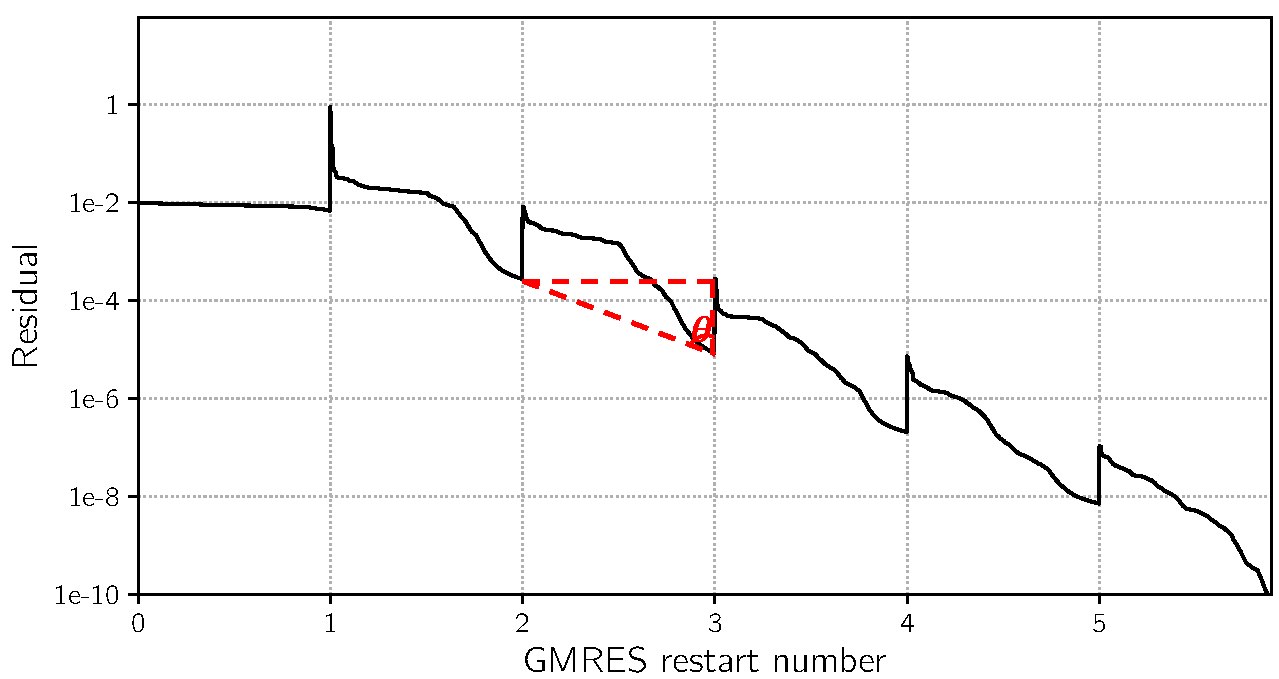
\includegraphics[width=0.99\linewidth]{fig/convergence_tuning.pdf}
	\caption{Heuristic of $lsa$ in UCGLE.}
	\label{fig:cos}
\end{figure}

It is necessary to select suitable value of $lsa$ for different linear systems. The autotuning proposed should be able to vary this parameter inside a given interval depending on several pre-defined critera. In this dissertation, we implement two modes of varying $lsa$, either starting from the a maximum or minimum value with a fixed length to decrease or increase for each time LS polynomial preconditioning.

\textbf{$1^{st}$ criterion:} The first criterion $cr_i$ is defined as follows, with $i$ indexing different times of restarting in GMRES Component. 

\begin{equation}
cr_i = \frac{||r_i||_2}{||r_{i-1}||_2}.
\end{equation}

This parameter is defined as a ratio between $||r_i||_2$ and $||r_{i-1}||_2$. $||r_i||_2$ and $||r_{i-1}||_2$ represent respectively the Euclidean norm of this and previous time restarting residual vector before the LS preconditioning, shown as Fig. \ref{fig:cos}. This criterion is defined to quantify the acceleration rate (see the slope of the red dashed line in Fig. \ref{fig:cos} which connects two restaring points) of UCGLE with previous value of $lsa$, and the modification of this parameter for this time of LS preconditioning should depend on the evalution of $cr_i$. $cr_i < 1$ signficates the convergence of GMRES component, and the smaller it is, the more signficant the acceleration will be. If $cr_i=1$, there is no convergence for last time $m$ steps of GMRES. If $cr_i > 1$ which means $||r_{i-1}||_2 > ||r_{i}||_2$, and the GMRES Component diverge. This first criterion is weak, which assures the convergence of GMRES, but it is impossible to control the acceleration rate by LS polynomial preconditioning.

\textbf{$2^{nd}$ criterion:} The second criterion $ratio_i$ is defined as follows, with $i$ indexing different times of restarting in GMRES Component.

\begin{equation}
ratio_i=\frac{||R_i||_2}{||r_{i}||_2}.
\end{equation}

This parameter is defined as a ratio between $||R_i||_2$ and $||r_i||_2$. $||R_i||_2$ represents the restarted residual norm after the LS polynomial preconditioning, shown as the peaks of the residual norms for the restartings in Fig. \ref{fig:cos}.  The parameter $ratio_i$ defines the amplification of LS residual norm over the residual norm before the preconditioning. In other words,  the value of $ratio_i$ determines the length of peaks in Fig. \ref{fig:cos}. In UCGLE, the peaks cannot be too large, if not the convergence will be solved down, and GMRES Component might easily obtain the divergence. The definition of this criterion gives an upper limit for the residual norm generated by LS polynomial preconditioning, and it will determines the value of parameter $lsa$ at runtime. This parameter can be seen as a strong factor to evaluate the quality of LS polynomial preconditioning.


\textbf{$3^{rd}$ criterion:} The third criterion $||R_i||_2$ is defined as follows, with $i$ indexing different times of restarting in GMRES Component.

\begin{equation}
||R_i||_2.
\end{equation}

The definition of this criterion is really simple, which is just the absolute residual norm generated by LS polynomial for each restarting. This parameter determines that the absolute norm of LS polynomial preconditioning should not be too enormous. The second criterion $ratio_i$ and  $||R_i||_2$ can be seen as a complementary for each other. The former defines a relative amplication of residual norm caused by $lsa$, and the latter introduces a roof for the absolute enlargement of this residual norm. The combination of the two critera can control the LS polynomial preconditioning norm always in a good situation, and avoid the possibility of slowing down or divergence. The good selection of threshold for them is really important.

\subsection{Heuristic and Autotuning Algorithm}

After the defintion of criteria, in this section, we present the heuristic and autotuning algorithm for selecting $lsa$ at runtime. We give respectively the algorithm and workflow in Algorithm \ref{alg:ucgle-autotuning} and Fig .\ref{fig:autoworkflow}. Before the introduction of the heuristic in details, we list the different parameters of autotuning are listed as below:

\begin{itemize}
	\item $lsa_{init}$: the initial pre-defined value of applied times of LS polynomial preconditioning, the automatic selection of $lsa$ at runtime will start from this value, by two different modes.
	\item $mode$: two modes to vary the value of $lsa$ at runtime:
	\begin{itemize}
		\item \textit{max}:  maximum mode which diminue $lsa$ starting from $lsa$.
		\item \textit{min}: min: minimum mode, $lsa_{max}$: for minimum mode.
	\end{itemize}
	\item $lsa_{min}$: the minimum value that $lsa$ should not break in \textit{max} mode.
	\item $lsa_{max}$: the maximum value that $lsa$ should not break in \textit{min} mode.
	\item $cr_i = \frac{||r_i||_2}{||r_{i-1}||_2}$: the $1^{st}$ criterion to control the convergence rate of GMRES Component. The threshold of this criterion can be prescribed by the users, which will define the acceptable of convergence rate. However, in this dissertation, we fix it to be $1$, which means this criterion separate only if GMRES Component converge or not.
	\item $ratio_i=\frac{||R_i||_2}{||r_{i}||_2}$: the $2^{nd}$ criterion to determine the length of peaks generated by LS polynomial preconditioning. This criterion the relative amplification of residual norm.
	\item $||R_i||_2$: the $3^{nd}$ criterion to determine the absolute amplification of residual norm produced by LS polynomial preconditioning.
	\item $ratio_{max}$: the threshold of $ratio_i$, and the acceptable value should not exceed it.  
	\item $norm_{max}$: the threshold of $||R_i||_2$, and the acceptable value should not exceed it. 
	\item $lsa_i$: the value of $lsa$ determined by the $1^{st}$ criterion $cr_i$ for the restart indexing by $i$. Hence, the initial given value $lsa_1 = lsa$.
	\item $\overline{lsa_{i}}$: the value of $lsa$ determined by the $2^{nd}$ criterion $ratio_i$ and $e^{rd}$ criterion $||R_i||_2$. Thus it is the final determined value which will be applied to the LS polynomial preconditioning.
	\item $length$: the step length to vary the value of $lsa$, either in \textit{max} or  \textit{min} mode.
	\item $m$: the Krylov subspace of GMRES Component. this parameter is fixed when autotuning $lsa$.
	\item $l$: the degree of LS polynomial. This parameter is also fixed to a given value for the autotuning of $lsa$.
\end{itemize}

\begin{algorithm}[htbp]{}
	\caption{GMRES Component Implementation for Autotuing UCGLE}   
	\label{alg:ucgle-autotuning}   
	\begin{algorithmic}[1]
		\Function {AT-UCGLE}{\textit{mode}, $lsa_{init}$, $lsa_{max}$, $lsa_{min}$, $length$, $norm_{max}$, $ratio_{max}$}
		\State $i=1$, $lsa_1 = lsa$ and give initial guess $x_0$
		%\State $r_0 = b - Ax_0$
		\While{not converged}
		%\State GMRES($A, x_{i-1}$)$\rightarrow x_i$ \label{gmres}
		\State $r_{i-1} = b - Ax_{x-1}$     \label{gmres}
		\State $r_i = b - A_{x_i}$, and $v_i = \frac{r_{i-1}}{||r_{i-1}||_2}$
		\For{$q = 1, 2, \cdots, m$}
		\State Compute $h_{p,q}=(Av_q, v_p)$ for $p = 1, 2, \cdots, q$
		\State Compute  $v_{q+1} = AV_q - \sum_{p =1}^{q}h_{p,q}v_p$,  $h_{q+1,q} = ||v_{q+1}||_2$, and $v_{q+1} = v_{q+1}/h_{q+1,q}$
		\EndFor
		\State $x_i = x_{i-1}+V_my_m$, with $y_m$ minimize $||\beta e_1 - H_my||_2$
		\If{use LSP preconditioning}
		
		
		\If{i > 1}
		\State $cr_i=\frac{||r_i||2}{||r_{i-1}||_2}$
		\If {$cr < 1$}
		\Switch{$mode$}
		\Case{max}
		\State $lsa_i = lsa_{init} - length \times (i - 1)$
		\If{$lsa_i < lsa_{min}$}
		\State $lsa_i =  lsa_{min}$
		\EndIf
		\EndCase
		\Case{min}
		\State $lsa_i = lsa_{init} + length \times (i - 1)$
		\If{$lsa_i > lsa_{max}$}
		\State $lsa_i =  lsa_{max}$
		\EndIf 
		\EndCase
		\EndSwitch
		\EndIf
		\EndIf
		\For{$j = 0, 1, \cdots, lsa_i - 1$} \label{lsastart}
		%\State LSP\_Iterator($l$)$\rightarrow res_j$
		\For {$i=k, 2, \cdots, l-1$}
		\State $\omega_{k+1}=\frac{1}{\beta_{k+1}}[A\omega_k-\alpha_k\omega_k-\delta_k\omega_{k-1}]$
		\State $x_{k+1}=x_k+\eta_{k+1}\omega_{k+1}$
		\EndFor 
		\State $x_i = x_i + x_l$
		\State $R_i = b - Ax_i$
		\State  $ratio=\frac{||R_i||_2}{||r_{i}||_2}$
		\If{$ratio < ratio_{max}$ and $||R_i||_2 < norm_{max}$}
		\State \textbf{continue}
		\Else
		\State $\overline{lsa_{i}}= j + 1$
		\State \textbf{break}
		\EndIf 
		\EndFor \label{lsaend}
		
		\EndIf
		
		\State $i = i + 1$
		\State Go to \ref{gmres} to restart GMRES
		\EndWhile
		\EndFunction
	\end{algorithmic}  
\end{algorithm}

After the introduction of parameters in the autotuning algorithm, here we present the autotuning scheme in details. This autotuning can be divided into two parts. This first part is to varying the value $lsa$ in either \textit{max} or \textit{min} mode according to the $1^{st}$ criterion $cr_i$. After a $m$-step GMRES indexing by $i$, if the convergence achieves, GMRES Component will exit. Otherwise, if LS polynomial preconditioning is not available, GMRES will be restarted in a standard way using $x_i$ as a initial vector for the next $m$-step GMRES. If the preconditioning is applicable, and $i=1$, the value of $lsa_1$ is given as $lsa_{init}$. For $i > 1$, the $lsa_{i-1}$ will be evaluated by calculating $cr_i$. If $cr_i < 1$, which means the GMRES with $lsa_{i-1}$ is able to converge. We can continue to try to generate a new $lsa_i$ based on the different modes. If the $lsa_i$ is  either too large or too small for the two modes, $lsa_i$ will be fixed to be $lsa_{min}$ and $lsa_{max}$, respectively. In a word, this part of autotuning will produce a value $lsa_i$ based on the condition of $cr_i$.

The second part of the autotuning is more imporant, since it is directly linked to the iterations of LS polynomial preconditioning. For each $i$, the loop from line \ref{lsastart} to \ref{lsaend} in Algorithm \ref{alg:ucgle-autotuning}, is the operation that applies $lsa_i$ times LS polynomial. In this loop, for each $j \in 0, 1, 2, \cdots, lsa_i - 1$, a temporary solution $x_l$ will be generated by a $l$ degree LS polynomial. Then $x_l$ will be continuously added to $x_i$. For each $j$, current residual $R_i$ can be defined as $b-Ax_i$, and a $ratio=\frac{||R_i||_2}{||r_{i}||_2}$ will also be calculated. If the condition that $ratio < ratio_{max}$ and $||R_i||_2 < norm_{max}$ are both satisfied at the same time, it means that both the peak and absolute residual norm sizes are acceptable. Thus the loop can continue until the end of loop. In this case, we have $\overline{lsa_i} = lsa_i$. If at least one of the two conditions cannot be satisfied, it means that either the peak size or the absolute residual LS polynomial preconditioning is too large, and the loop will be immediately broken. In this case, we $\overline{lsa_i} < lsa_i$. In summary, the real value of $lsa$ for the LS polynomial preconditioning is $\overline{lsa_i}$. The combination of criteria $ratio_i$ and $||R_i||_2$ can really select the good value of $lsa_i$ at runtime, which assures the rapidest convergence produced by LS polynomial precondtioning.

\begin{figure}[t]
	\centering
	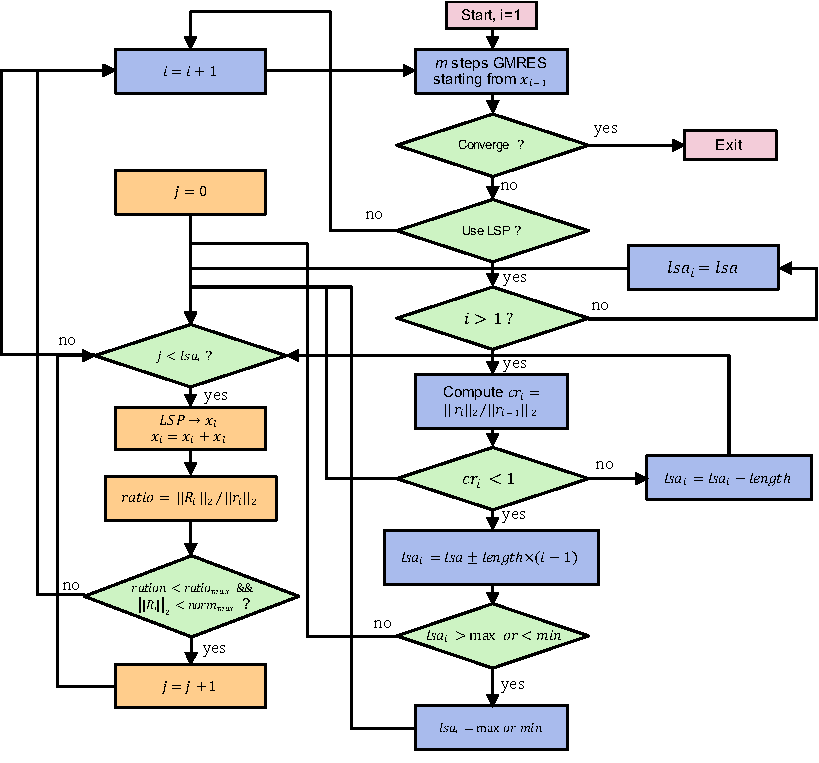
\includegraphics[width=0.99\linewidth]{fig/autotuning-workflow.pdf}
	\caption{Autotuning workflow for UCGLE.}
	\label{fig:autoworkflow}
\end{figure}

\subsection{Experiments}

After the proposition of heuristic, we will evaluate this autotuning scheme in this section.

\subsubsection{Test Methods Setting}

Since we have evaluated the influence of different parameters on the convergence using the test matrix $utm300$ from the Matrix Market collection, we continue to use it for the autotuning tests. The Krylov subspace size $m$ for GMRES Component in different methods is fixed as $90$, and the degree of LS polynomial is set to be $10$. The parameters $length$, $ratio_{max}$, $norm_{max}$ are respectively given as $2$, $1.0\times10^{5}$ and $1.0\times10^{4}$ for UCGLE with autotuning scheme (denote it as AT-UCGLE). We list the test methods as below.

\begin{itemize}
	\item UCGLE($lsa=4$): UCGLE implementation without autotuning scheme, and $lsa=4$;
	\item UCGLE($lsa=10$): UCGLE implementation without autotuning scheme, and $lsa=10$;
	\item UCGLE($lsa=20$):  UCGLE implementation without autotuning scheme, and $lsa=20$;
	\item AT-UCGLE(max, $lsa=20$): UCGLE implementation with autotuning scheme, varying the value of $lsa$ in \textit{max} mode, and initial value of $lsa$ is set to be $20$;
	\item AT-UCGLE(max, $lsa=30$): UCGLE implementation with autotuning scheme, varying the value of $lsa$ in \textit{max} mode, and initial value of $lsa$ is set to be $30$;
	\item AT-UCGLE(min, $lsa=4$):  UCGLE implementation with autotuning scheme, varying the value of $lsa$ in \textit{min} mode, and initial value of$lsa$ is set to be $4$.
\end{itemize}
	\begin{figure}
		\centering
		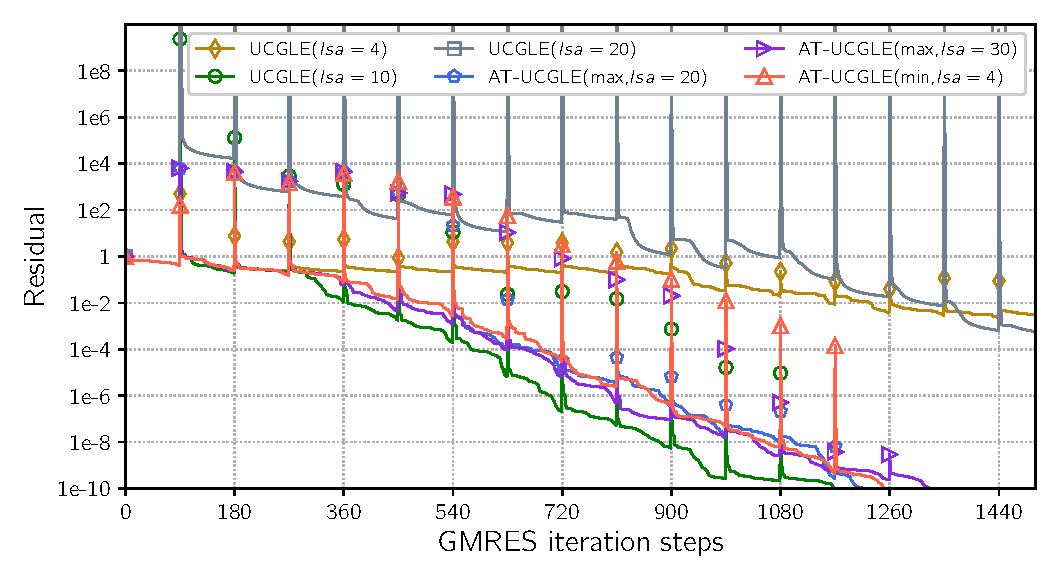
\includegraphics[width=0.99\linewidth]{fig/autotuning.eps}
		\caption{Convergence Comparison for UCGLE with and without Autotuning.}
		\label{fig:autotuning}
	\end{figure}

\subsubsection{Convergence Comparison}

The convergence comparison for UCGLE with and without autotuning is given as Fig. \ref{fig:autotuning}. In this figure, firstly we can find that UCGLE($lsa=10$) has the fastest convergence. However, it is difficult for UCGLE($lsa=4$) and UCGLE($lsa=20$) to achieve the convergence. For the former, the peak for each restarting is relative small, and the acceleration of LS polynomial preconditioning is weak. For the latter, the absolute norm of restart residual generated by LS polynomial is too large which exceeds $1.0\times10^{15}$, and it is also difficult for UCGLE to quickly converge. It is not marked in Fig. \ref{fig:autotuning}, but a large number of tests indicate that $lsa=10$ is the best value for UCGLE without preconditioning if all the other parameters are fixed.

In practice, for a given application, the users have no idea to directly select the best value for $lsa$. Thus the autotuning scheme is proposed to automatically select the best value inside a given interval at runtime. For AT-UCGLE(max, $lsa=20$) and AT-UCGLE(max, $lsa=30$) which start the iterations with a very large $lsa_{init}$ (respectively $20$ and $30$), they can obtain the convergence much more quickly than UCGLE($lsa=20$). They a little more steps for the convergence comparing the best case UCGLE($lsa=20$). For AT-UCGLE(min, $lsa=4$) which starts the iteration with a small pre-defined $lsa_{init}=4$, its iteration steps for convergence is also competitive with the best case UCGLE($lsa=20$). For AT-UCGLE in \textit{max} starts from a very large $lsa_{init}$, it will produce an enormous residual normal which damanges the convergence (see UCGLE($lsa=20$ in Fig. \ref{fig:autotuning})). The constraint of $||R_i||_2$ can ensure this norm always in an acceptable condition, and the speedup of convergence is obvious. In a word,  two modes of varying $lsa$ are both effective to approximate the best numerical performance with a too large or small prescribed $lsa_{init}$.

\begin{table}[htbp]
	\renewcommand{\arraystretch}{1.4}
	\small	
	\caption{Iteration steps and Time Comparison.}
	\label{table:autotuning}
	\centering
	\begin{tabular}{c|c|c|c|c}
		\toprule
		\cellcolor{gray!50}Methods & \cellcolor{gray!50}Iterations & \cellcolor{gray!50}Iteration Effectiveness&\cellcolor{gray!50}Time (s) & 	\cellcolor{gray!50}Time Effectiveness\\
		\midrule
		UCGLE($lsa=10$)  & $1169$ & 100\%& $0.35$ &100\%\\
		\cellcolor{gray!20}UCGLE($lsa=4$) & \cellcolor{gray!20}$2513$ & \cellcolor{gray!20}46.5\%& \cellcolor{gray!20}$0.72$  &\cellcolor{gray!20}48.6\% \\
		UCGLE($lsa=20$) & $3226$ &36.2\%& $1.08$& 32.4\%\\
		\cellcolor{gray!20}AT-UCGLE(max, $lsa=20$) & \cellcolor{gray!20}$1220$ & \cellcolor{gray!20}95.8\%& \cellcolor{gray!20}$0.36$ &\cellcolor{gray!20}97.2\%\\
		AT-UCGLE(max, $lsa=30$)  &$1328$ & 88\%&$0.41$ &85.3\% \\
		 \cellcolor{gray!20}AT-UCGLE(min, $lsa=4$) &  \cellcolor{gray!20}$1252$ & \cellcolor{gray!20}93.4\%&  \cellcolor{gray!20}$0.38$ &\cellcolor{gray!20}92.1\%\\
		
		\bottomrule
	\end{tabular}
\end{table}

Table. \ref{table:autotuning} shows the exact number of iterations and execution for different methods. Moreover, both the effectiveness of iterations and time are also given in this table. The iteration effectiveness is defined as the ratio between the iteration number of the best case UCGLE($lsa=10$) and the one of the method to be compared. The time effectiveness can be also defined in a similar way. In this table, we can find that AT-UCGLE(max, $lsa=20$) achieve 95.8\%  iteration effectiveness and 97.2\% time effectiveness. AT-UCGLE(min, $lsa=4$) can achieve respectively 93.4\% and 92.1\% for the iteration and time effectiveness. The effectiveness of iteration and time for AT-UCGLE(max, $lsa=30$) are respectively 88\% and 85.3\%.

In summary, two modes are both useful with high iteration and time effectiveness comparing with the best case of UCGLE without autotuning. However, the selection of $lsa_{init}$ value is still a factor which influences the convergence. In \textit{max} mode, if $lsa_{init}$ is extreme large, the effectiveness might be a little low. That is the reason that AT-UCGLE(max, $lsa=30$) achieves only 88\% iteration effectiveness, but AT-UCGLE(max, $lsa=20$) can achieve about 95.8\%.

\subsubsection{Analysis}

The autotuning scheme proposed in this dissertation is able to selection a good value of the parameter $lsa$ in two steps for each time LS polynomial preconditioning. For each restarting indexing $i$, the first step is to generate a $lsa_i$ using a simple heuristic based on $cr_i$. This parameter can ensure the convergence for the next $m$-steps GMRES not worse than the previous one, but it cannot make decision for the speedup of LS polynomial preconditioning, which is the kernel of UCGLE. The second step is to select a best $\overline{lsa_i}$ according $ratio_i$ and $||R_i||_2$. Table \ref{table:autotuning2} gives the comparsion of $lsa_i$ and related $\overline{lsa_i}$ at each restarting inside AT-UCGLE. In this table, we can find the benefits of the criteria $ratio_i$ and $||R_i||_2$, which can limit the value of $lsa_i$ in a good situation.

\begin{table}[htbp]
	\renewcommand{\arraystretch}{1.4}
	\footnotesize	
	\caption{$lsa_i$ vs $\overline{lsa_i}$ for each restart in AT-UCGLE.}
	\label{table:autotuning2}
	\centering
	\begin{tabular}{c|c|c|c|c|c|c|c|c|c|c|c|c|c|c}
		\toprule
		\cellcolor{gray!50}Methods & \cellcolor{gray!50}1 & \cellcolor{gray!50}2&\cellcolor{gray!50}3&\cellcolor{gray!50}4&\cellcolor{gray!50}5&\cellcolor{gray!50}6&\cellcolor{gray!50}7 &\cellcolor{gray!50}8&\cellcolor{gray!50}9&\cellcolor{gray!50}10&\cellcolor{gray!50}11&\cellcolor{gray!50}12&\cellcolor{gray!50}13&\cellcolor{gray!50}14\\
		\midrule
		AT-UCGLE(max, $lsa=20$)  $lsa_{i}$&$20$&$18$ &$16$&$14$&$12$&$10$&$8$&$6$&$4$&$4$&$4$&$4$&$4$&\\
		\cellcolor{gray!20}AT-UCGLE(max, $lsa=20$) $\overline{lsa_{i}}$& \cellcolor{gray!20}$5$ & \cellcolor{gray!20}$8$&\cellcolor{gray!20}$8$&\cellcolor{gray!20}$9$&\cellcolor{gray!20}$10$&\cellcolor{gray!20}$8$&\cellcolor{gray!20}$6$&\cellcolor{gray!20}$6$&\cellcolor{gray!20}$4$&\cellcolor{gray!20}$4$&\cellcolor{gray!20}$4$&\cellcolor{gray!20}$4$&\cellcolor{gray!20}$4$&\cellcolor{gray!20}  \\
		AT-UCGLE(max, $lsa=30$) $lsa_{i}$& $30$ & $28$&$26$&$24$&$22$&$20$&$18$&$16$&$14$&$12$&$10$&$8$&$6$&$4$   \\
		\cellcolor{gray!20}AT-UCGLE(max, $lsa=30$)  $\overline{lsa_{i}}$&\cellcolor{gray!20}$5$&\cellcolor{gray!20}$8$ &\cellcolor{gray!20}$8$&\cellcolor{gray!20}$9$&\cellcolor{gray!20}$10$&\cellcolor{gray!20}$10$&\cellcolor{gray!20}$10$&\cellcolor{gray!20}$10$&\cellcolor{gray!20}$11$&\cellcolor{gray!20}$10$&\cellcolor{gray!20}$10$&\cellcolor{gray!20}$8$&\cellcolor{gray!20}$6$&\cellcolor{gray!20}$4$\\
		AT-UCGLE(min, $lsa=4$) $lsa_{i}$& $4$ & $6$&$8$&$10$&$12$&$14$&$16$&$18$&$20$&$22$&$24$&$26$&$28$&    \\
		\cellcolor{gray!20}AT-UCGLE(min, $lsa=4$) $\overline{lsa_{i}}$&\cellcolor{gray!20}$4$ &\cellcolor{gray!20}$6$&\cellcolor{gray!20}$8$&\cellcolor{gray!20}$10$&\cellcolor{gray!20}$11$&\cellcolor{gray!20}$10$&\cellcolor{gray!20}$9$&\cellcolor{gray!20}$11$&\cellcolor{gray!20}$10$&\cellcolor{gray!20}$11$&\cellcolor{gray!20}$11$&\cellcolor{gray!20}$10$&\cellcolor{gray!20}$11$&\cellcolor{gray!20}    \\
		
		\bottomrule
	\end{tabular}
\end{table}

\section{Conlusion}

In this chapter, we inverstigate the different autotuning modes for the iterative methods. We implement an automatic contectual selection scheme for the selected parameter of UCGLE. This autotuning heuristic is established with the definition of multiple level criteria and a workflow for the selection of best value for parameters at runtime. The effectiveness of proposed autotuning scheme is proved by the experimental results. In the future, a more flexible workflow should be proposed to vary the value inside a given interval. Moveover, UCGLE has a large number of parameters which have impact on his numerical and parallel performance. Thus the autotuning scheme should be studied. The final goal is to implement an adaptive verison of UCGLE, which can autotune various parameters at the same time.

\clearemptydoublepage